\section{Background}
\label{sec:background}

We provide a brief background about unmanned aerial vehicles (UAVs). 
%In \Sec{sec:uav}, we present the lay of the land, discussing the different types of UAV tiers. 
In \Sec{sec:mav}, we discuss the most ubiquitous and growing segment of UAVs, i.e., Micro Aerial Vehicles (MAVs) and its different flight-wing types. In  \Sec{sec:constraints}, we present the overall system level constraints facing MAVs.

\begin{comment}
\subsection{Unmanned Aerial Vehicle (UAV) Tiers}
\label{sec:uav}

There is no single established standard to categorize all drones. However, certain high-level characteristics such size as weight, and range, all of which ultimately determine the drone use case, can be used as the base for such clustering. Table~\ref{nato-classification-drones} shows one such proposed classification guide provided by NATO. This classification allows drones to be specified based on the altitude and range which missions require.

Drones, otherwise known as Unmanned Aerial Vehicles (UAVs), initially emerged as military weapons to be mainly deployed for missions in which having a human pilot will be a disadvantage~\cite{rs}. It is not until recently that there has been a significant proliferation of Micro Aerial Vehicles (MAV) for civilian applications, such as crop surveying, industrial fault detection, mapping, surveillance and aerial photography. 


\begin{table}[t!]
\vspace{5pt}
\centering
\caption{UAVs by NATO Joint Air Competence Power~\cite{nato-uav-classification}.}
\label{nato-classification-drones}
\resizebox{\columnwidth}{!}{
\begin{tabular}{|c|c|c|c|}
\hline
Category                                                              & Weight (kg) & Altitude (ft) & Mission Radius (km) \\ \hline\hline
Micro                                                                 & \textless2                                             & \textless200                                                                    & 5                                                                           \\ \hline
Mini                                                                  & (2-20)                                                 & (200- 3000)                                                                     & 25                                                                          \\ \hline
Small                                                                 & (20-150)                                               & (3000-5000)                                                                    & 50                                                                          \\ \hline
Tactical                                                              & (150-600)                                              & (5000-10000)                                                                    & 2000                                                                        \\ \hline
Combat & \textgreater600                                        & \textgreater10000                                                               & Unlimited                                                                   \\ \hline
\end{tabular}
}
\end{table}


\begin{comment}
\begin{table}[]
\centering
\caption{Classification based on Size}
\label{my-label}
\begin{tabular}{|l|l|}
\hline
\textbf{Size} & \textbf{Value}  \\ \hline
Very Small    & 30 to 50 cm     \\ \hline
Small         & 50 to 2 m       \\ \hline
Medium        & 5 to 10 m       \\ \hline
Large         & \textgreater10m \\ \hline
\end{tabular}
\end{table}
\begin{table}[]
\centering
\caption{Classification of UAV based on Range and Endurance}
\label{my-label}
\begin{tabular}{|l|l|l|}
\hline
\textbf{Class}   & \textbf{Range} & \textbf{Endurance}    \\ \hline
Very Close Range & 5 Km           & 20-45 min             \\ \hline
Close Range      & 50 Km          & 1 to 6 Hours          \\ \hline
Short Range      & 150 Km         & 8 to 12 Hours         \\ \hline
Mid Range UAV    & 650 Km         & 12 to 36 Hours        \\ \hline
Endurance UAV    & 300 Km         & \textgreater 36 Hours \\ \hline
\end{tabular}
\end{table}
\end{comment}

\subsection{Micro Aerial Vehicles (MAV)}
\label{sec:mav}
There is no single established standard to categorize all drones. However, typically, a UAV is classified as a ``Micro UAV'' if its weight is less than 2~\si{\kilo\gram}, and it operates within a radius of 5~\si{\kilo\meter}. MAVs' small size increases their accessibility and affordability by shortening their ``development and deployment time,'' as well as reducing the cost of ``prototyping and manufacturing''~\cite{Zhang2017207}. Furthermore, their small size coupled with their ability to move flexibly empowers them with the agility and maneuverability necessary for various applications, such as sports photography, indoor mapping, surveillance, etc.

MAVs come in different shapes and sizes. A key distinction is their wing type. On one end of the spectrum, MAVs have fixed wings. On the other end, MAVs have rotor wings. Fixed wing MAVs, as their names suggest, have fixed winged airframe. Their wing structure is deployed for taking-off, navigation, and landing. These MAVs typically require (small) runways for taking-off and landing. Due to the aerodynamics of their wings, they are capable of gliding in the air, which improves their ``endurance'' (i.e., how long they last in the air).

Rotor wing MAVs are becoming the dominant kind. They take off vertically, land vertically, and move with more agility compared to their fixed-wing counterparts. They do not require constant forward airflow movement over their wings from external sources since they generate their own thrust using rotors. Such capabilities enhance their benefits in constrained environments, especially indoors, such as in buildings and warehouses where there are many tight spaces and corners.

Although MAVs enjoy the aforementioned advantages, their complex mechanical (rotors/payload etc) and electrical subsystem (battery, processors) limit their endurance, and as such present unique challenges for system architects and engineers.

\begin{figure}[t!]
\centering
    \begin{subfigure}{.49\columnwidth}
    \centering
    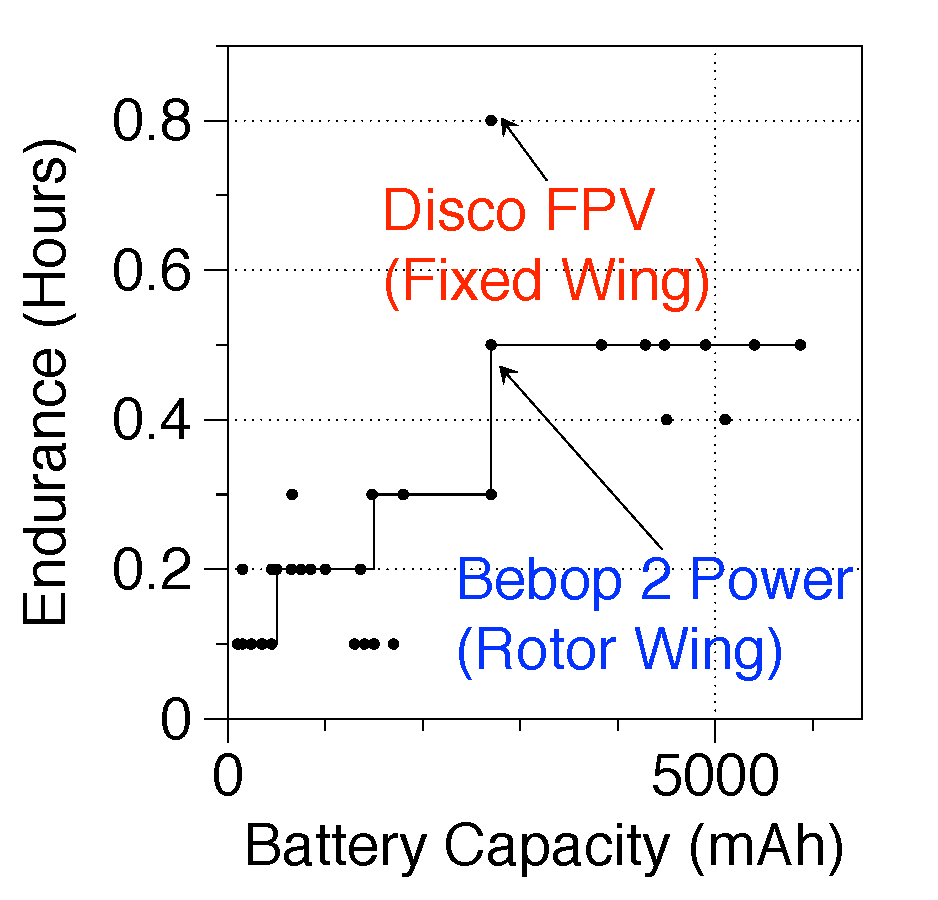
\includegraphics[trim=0 0 0 0, clip, width=0.9\columnwidth]{figs/Battery_Capacity_vs_Endurance_plot}
   \vspace{-5pt}
   \caption{Flight endurance time plotted against total battery capacity.}
    \label{fig:battery_capacity_vs_endurance}
    \end{subfigure}
    \hfill
    \begin{subfigure}{.49\columnwidth}
    \centering	
    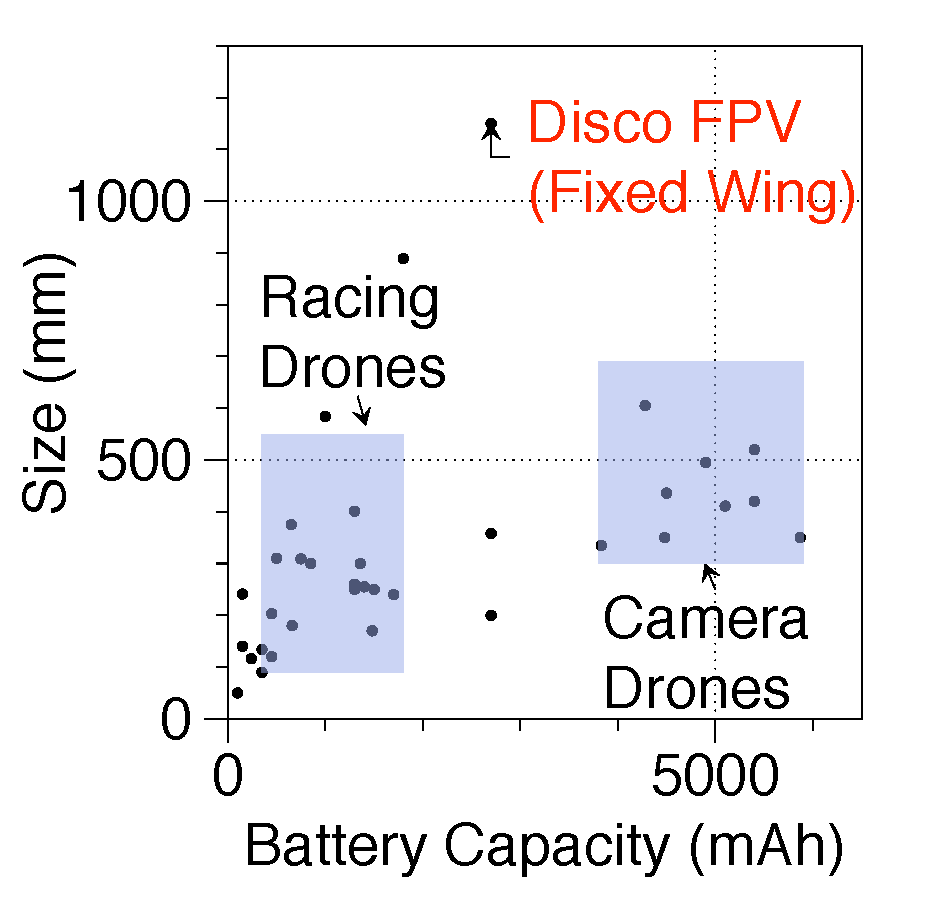
\includegraphics[trim=0 0 0 0, clip, width=0.9\columnwidth]{figs/Size_vs_Battery_Capacity}
    \vspace{-5pt}
    \caption{Drone size plotted against total battery capacity.}
    \label{fig:battery_capacity_vs_size}
    \end{subfigure}
\caption{MAVs based on battery capacity and size. Endurance is important for MAVs to be useful in the real-world. However, their small size limits the amount of on-board battery capacity.}
\label{fig:tradeoff}
\end{figure}

\begin{comment}

\subsection{rotor-based Micro Aerial Vehicles: UAV of choice}
%Among the aforementioned categories, rotor-based Micro aerial vehicle have an outburst of attention in recent years. This section elaborates how their rotor-based flight mechanism and smaller size can explain such a trend.

\textit{rotor based flight mechanism:} Using their flight mechanism, one can classify UAVs to fixed wing, flapping wing, or rotary wing. Though fixed-wings "simpler structure and more efficient aerodynamics provide the advantage of longer flight"(http://www.uavinsider.com/rotary-wing-vs-fixed-wing-uavs/),  the aircrafts with rotors are capable of "
%vertically taking off and landing, fixed-point hovering, flying
at low level altitude, and great stability and maneuverability."~\cite{Development-of-a-Micro-Aerial-Vehicle}. 

\textit{small size:} MAVS are aircrafts of size less than 15 cm length, width, or height and weigh less than 100 g. Such a small size have increased accessibility and affordibily of such systems by shortening the "development and deployment time", and reducing the cost for "prototyping and manufacturing", ~\cite{Rugged Embedded Systems 1st Edition book}. 
In addition, the combination of the small size and the hovering capability of the rotors provide these systems with the agility and  maneuverability necessary for various applications such as sports photography, indoor mapping, surveillance and etc.
\end{comment}

%Micro-Aerial Vehicles(MAV) comes in different shapes and sizes. On one end of the spectrum, MAV have fixed wing. On the other end, we have rotor based. Both these type of MAV can have electric motors or internal combustion engine as the propulsion system. The choice of propulsion system has a direct impact on the range and endurance of the MAV. There are also hybrid MAVs which uses both electric and internal combustion engine for propulsion. 

\begin{comment}
\begin{table}
\centering
\resizebox{\columnwidth}{!}{%
\caption{Drone categories.}
\label{tab:drones}
\begin{tabular}{|l|l|l|l|l|}
\hline
Category          & weight & range(km) & endurance(h) & altitude(h)     \\ \hline\hline
Micro       \textless2      &  \textless1      &           & 5-30 min     & \textless330 \\ \hline
Mini              &  \textless1 &           & 1-2          &              \\ \hline
Small             &    \textless13.5    &           &              &              \\ \hline
Light/ultra Light &     \textless242   &           &              &              \\ \hline
Normal            &   \textless4332     &           &              &              \\ \hline
Large             &     \textless4332   &           &              &              \\ \hline
\end{tabular}
}
\end{table}
\end{comment}

\begin{comment}
\subsection{Drone Platforms}
\label{ssec:drone-arch}
\begin{table}[]
\centering
\caption{Drone tiers: this table will contain high level ideas about drones from the pure functionality level, i.e. no system design perspective. e.g frame size, flight time, max speed, avg payload, max payload}

\label{my-label}
\begin{tabular}{|l|l|}
\hline
Drone Type & Frame size {[}mm{]} \\ \hline
Nano       & 80-100              \\ \hline
Micro      & 90-180 mm           \\ \hline
Mini       & 150-300             \\ \hline
\end{tabular}
\end{table}
Table~\ref{tab:drone-platforms}
\begin{table*}[t!]
\centering
\caption{Drone platform characteristics. pick a drone from different tiers and introduce the specs (from system perspective)}
\label{tab:drone-platforms}
\begin{tabular}{ |p{3cm}||p{3cm}|p{3cm}|p{3cm}|  }
 \hline
 Name     or Area Name& A nano drone name & a micro drone name & a mini drone name \\
 \hline
Power   & AF    &AFG&   004\\
Flight-time &   AX  & ALA   &248\\
Battery &AL & ALB&  008\\
FMU    &DZ & DZA&  012\\
Payload &   AS  & ASM&016\\
... & AD  & AND   &020\\
Companion computer & AO  & AGO&024\\
 \hline
\end{tabular}
\end{table*}
\end{comment}

\begin{comment}
\subsection{System Architecture old}
\label{ssec:drone-arch}

\red{in this section we explain the general architecture of a drone, since all the drones generally follow the same subsystem design. this is basically about the system architecture that is used by all the drones. explain the components within and how they interact etc.}

A typical autonomous MAV is equipped with an on-board computer, a flight controller, a collection of sensors, and a set of mechanical components including propellers and motors.

\paragraph{On-board Computer} A drone requires an on-board computer for autonomous flight. This on-board computer is responsible for high-level flight control and for computations that are not directly related to flight such as object detection or machine learning.

\paragraph{Flight controller} The flight controller is a microcontroller that handles a variety of low-level flight-related tasks. For example, it stabilizes the drone during flight, logs flight data, and controls the drone's orientation and speed to move it in the fashion specified by the on-board computer.

\paragraph{Sensors} Drones have the capability of gathering a rich set of sensory data, and the sensors they are equipped with will vary depending on the application that they are intended for. At minimum, however, a typical autonomous drone will be equipped with a sensor, such as an inertial measurement unit, that detects orientation, a sensor, such as a barometer or ultrasonic sensor, that detects altitude, and a sensor, such as a GPS receiver or optical flow camera, that detects position. There are many other possible sensors that may be attached to drones such as LIDAR sensors for 3-D mapping, cameras for photography, or even multispectral sensors for the purpose of monitoring crop health.

\paragraph{Other} In addition to sensors and processors, drones are composed of mechanical components such as motors, propellers, and frames.

\begin{figure}[h]
\centering
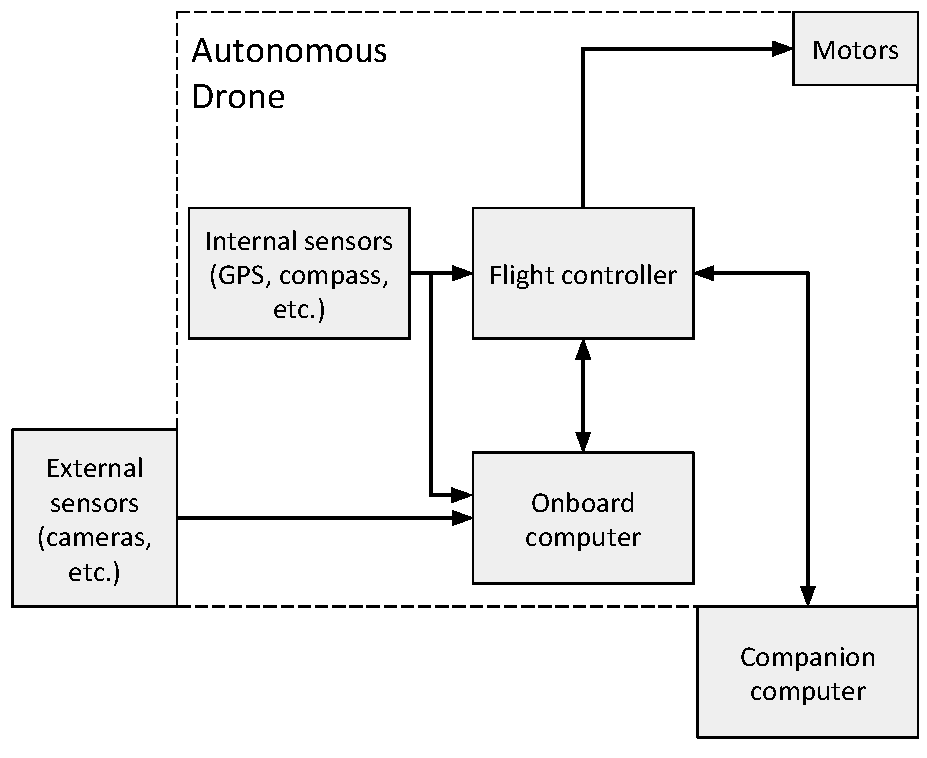
\includegraphics[width=\linewidth]{figs/drone-arch}
\caption{Architectural overview of our drone platform.}
\label{fig:dronearch}
\end{figure}
\end{comment}

\subsection{MAV Constraints}
\label{sec:constraints}

MAVs are tightly constrained on their resources. These constraints typically have to do with the limitations in the mechanical subsystems (rotors/payload size etc.) and the electrical subsystem (battery/processor etc.). For example, in package delivery, the payload size (i.e., the package) affects the mechanical subsystem, requiring more thrust from the rotors and this, in turn, affects the electrical subsystem by demanding more energy from the battery source. Comprehending these constraints is crucial to understand how to optimize the system. The biggest of the constraints as they relate to computer system design are performance and energy.

%At the high level, application (package delivery) requirements (lifting certain payload size for a certain range) turns into mechanical (rotors/motors thrust) and energy source (LIPO battery capacities) constraints. In turn, such constraints manifest themselves as performance and power constraints for architects to deal with. In this section we iterate over such constraints:

\paragraph{Performance Constraints:} MAVs are required to meet various real-time constraints. For example, a drone flying at a high speed looking for an object requires fast detection kernels. Such a task is challenging in nature for large-sized drones that are capable of carrying high-end computing systems, and they are virtually impossible on smaller sized MAVs. Hence, the stringent real-time requirements dictate the type of compute engines that can be put on these MAVs.

\paragraph{Energy Constraints:} The amount of battery capacity on board plays an important role in the type of applications MAVs can perform. Battery capacity has a direct correlation with the endurance of these vehicles. To understand this relationship, we show the most popular MAVs available in the market and compare their battery capacity to their endurance. As \Fig{fig:battery_capacity_vs_endurance} shows, higher battery capacity translates to higher endurance. We see a step function trend, i.e., for classes of MAVs that has similar battery capacity, they have similar endurance. On top of this observation, we also see that for the same battery capacity, a fixed wing has longer endurance compared to rotor based MAVs. For instance, in \Fig{fig:battery_capacity_vs_endurance}, we see that the Disco FPV (Fixed wing) has higher endurance compared to the Bebop 2 Power (Rotor wing) even though they have a similar amount of battery capacity.
Note that the size of MAV also has a correlation with battery capacity as shown in \Fig{fig:battery_capacity_vs_size}. 
%\red{I don't see how this discussion is relavant at all to architects. There should be at least one pointer we'll that connects this paragraph to architects}

\begin{comment}
\begin{figure}[t!]
\centering
\tabskip=0pt
    \begin{subfigure}{\columnwidth}
    \centering
    \vspace{0.1in}
    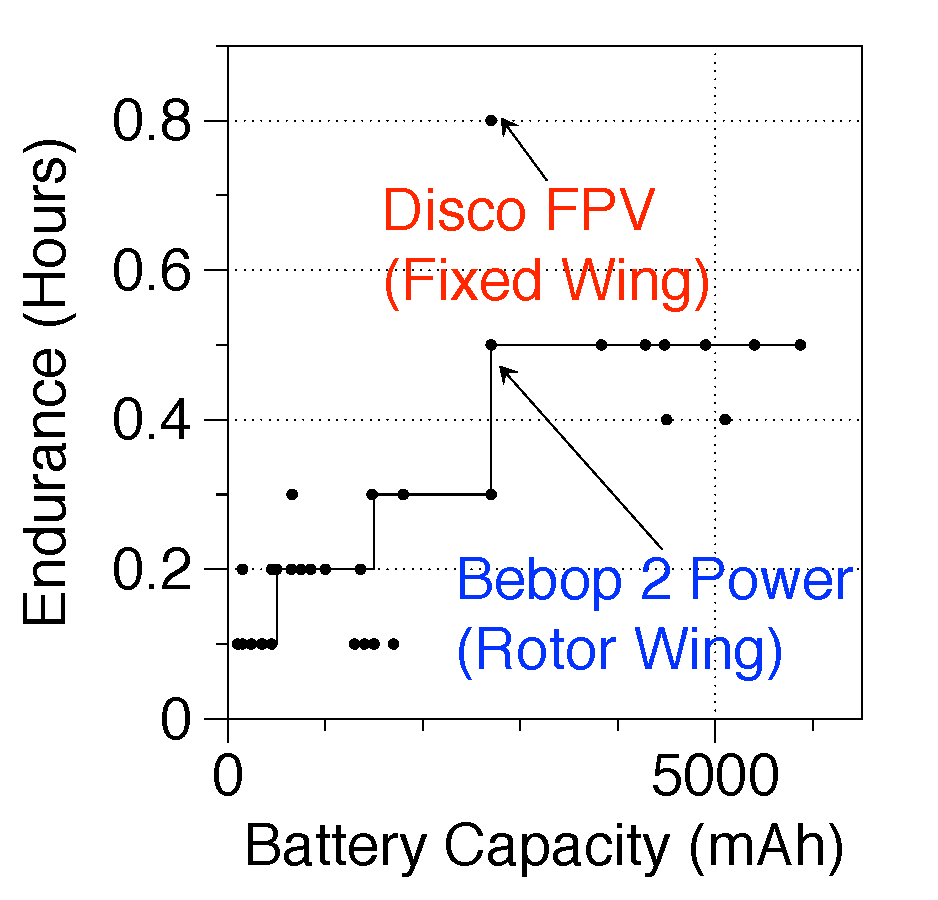
\includegraphics[trim=0 0 0 0, clip, width=.9\columnwidth]{figs/Battery_Capacity_vs_Endurance_plot}
    \caption{Endurance versus battery capacity.}
    \label{fig:battery_capacity_vs_endurance}
    \end{subfigure}
    \begin{subfigure}{\columnwidth}
    \centering
    \vspace{0.1in}
    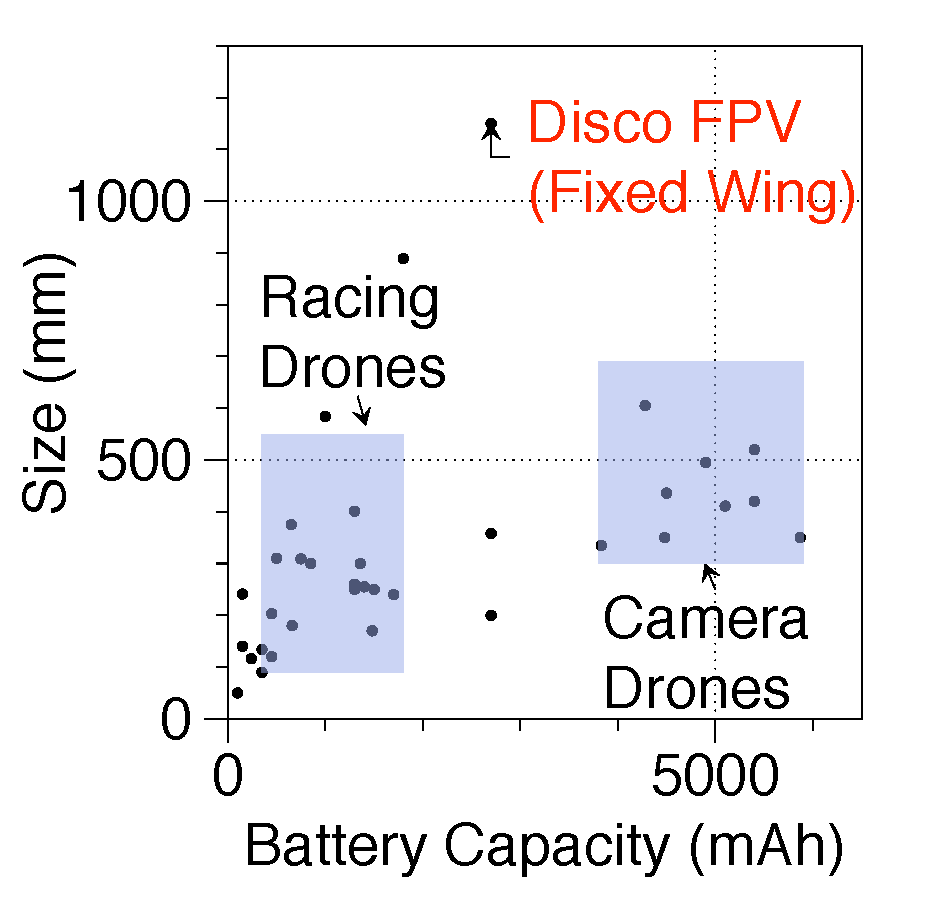
\includegraphics[trim=0 0 0 0, clip, width=.9\columnwidth]{figs/Size_vs_Battery_Capacity}
    \caption{Size versus battery capacity.}
    \label{fig:battery_capacity_vs_size}
    \end{subfigure}
\caption{MAVs based on battery capacity and size. Endurance is important for MAVs to be useful in the real-world. However, their small size limits the amount of on-board battery capacity.}
\label{fig:tradeoff}
\end{figure}
\end{comment}
%\red{I don't think we need the following two constraints. They are not relavant to architects, or if they are, it's hard to argue. also get rid of the figure that comes with it}
%\paragraph{Size:}The Size of MAV plays an important role in selection of mechanical and electrical subsystem. \Fig{fig:battery_capacity_vs_size} shows the distribution of size of MAVs and the battery capacity. MAVs deployed for aerial photography/surveying have higher battery capacity for their sizes. The racing MAVs are much smaller in size compared to camera MAVs but have more battery capacity for their size. However, racing MAVs typically have lower flight times in the order five to ten minutes because all the energy is spent generating higher thrusts.

%\red{this paragraph is confusing. where are the aerial photography/scanning drones in the figure. Are they camera drones? also it doesn't seem like we are discussing size constraints, but rather the implications of picking a size. also I think we should get rid of this or combine it with weight and imply the }

%\paragraph{Weight:} MAV weight, inclusive of its payload weight, can also have a significant impact on its endurance. Higher payload puts stress on the mechanical subsystems requiring more thrust to be generated by the rotors for hovering and maneuvering. This significantly reduces the endurance of MAVs. For instance, it has been shown that adding a payload of approximately 1.3~\si{\kilo\gram} reduces flight endurance by 4X~\cite{hasan2016sensorcloud}.


%Since most of the above-mentioned constraints either leads to performance bottlenecks in compute or energy consumption, opening up interesting avenues for research in computer architecture.\red{<- wording doesnt make sense. I also see the connection to compute architects.} To address these problems, computer architects need tools that extend beyond traditional simulators. 

%The aforementioned constraints opens up interesting avenues for research in computer architecture. To address these problems, computer architects need tools that extend beyond traditional simulators.



%Weight constraint is essential to the functioning of the aircrafts such as taking-off and stability. However, it has system implications. For example, it can throttle the system's thermal power budget since the added weight associated with introducing a fan might not be a possibility
%As was dicussed , the need to be mobile with high exploratory capacities constraints aerial agents to their amount of energy on board. (possibly cite one platform with flight time). As a result, longer flight time due to lower system performance can cause system to run out of energy and hence fail its mission. Performance improvements such as decreasing the decision making time (while drone hovers\footnote{one can think of this analogous to reduction of processor idle times}), or increasing decisions optimality (e.g. shorter paths to take while navigating) allows such systems to stay within energy budget. 

%\begin{figure}[t!]
%\centering
%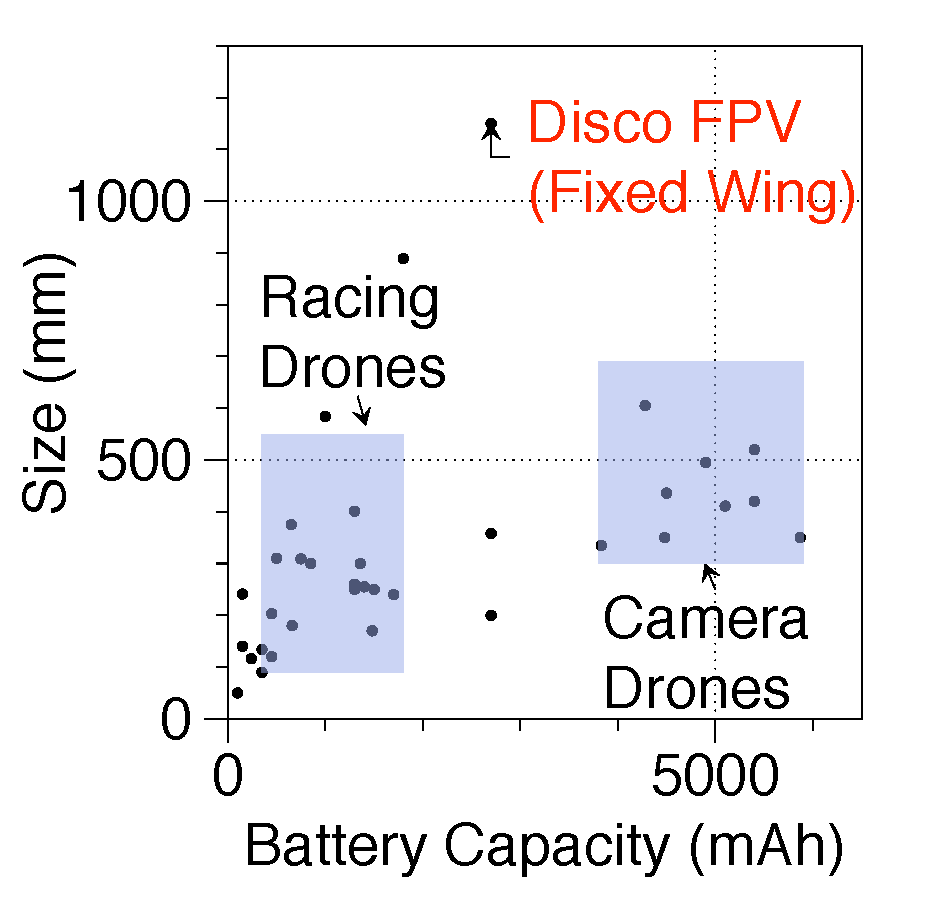
\includegraphics[width=0.5\columnwidth]{figs/Size_vs_Battery_Capacity}
%\vspace{-.4ex}
%\caption{ }
%\vspace{-3ex}
%\label{fig:1}
%\end{figure}

%\begin{figure}[t!]
%\centering
%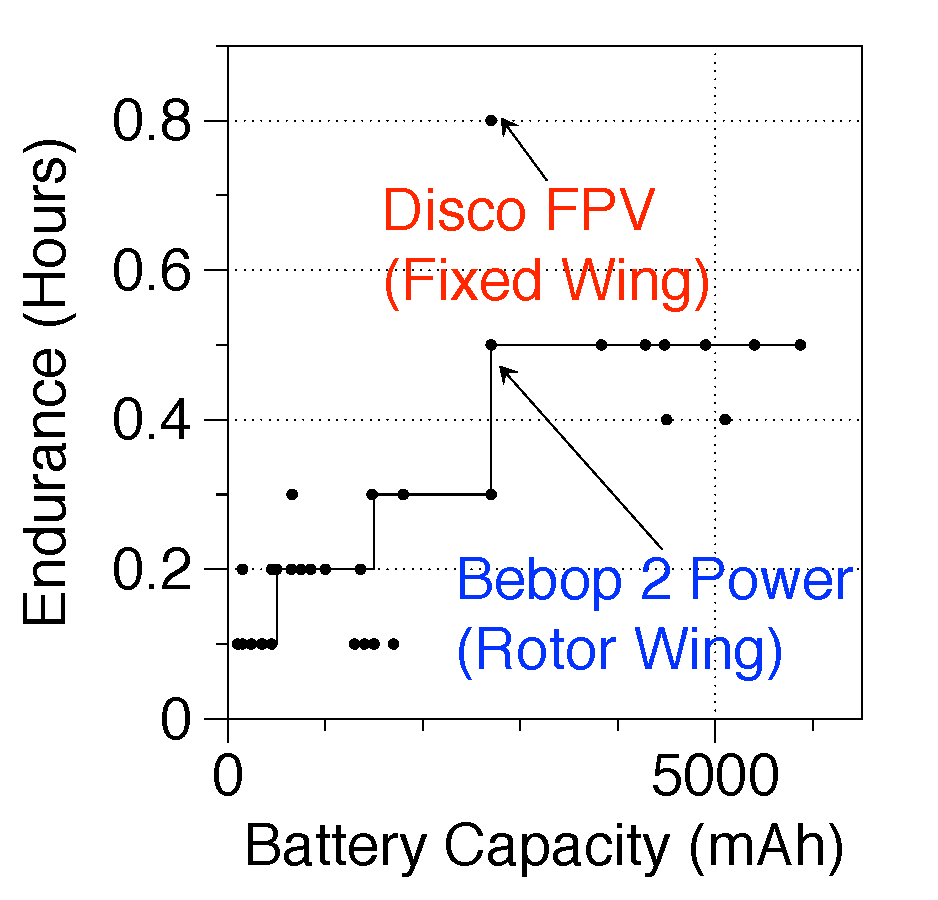
\includegraphics[width=0.5\columnwidth]{figs/Battery_Capacity_vs_Endurance_plot}
%\vspace{-.4ex}
%\caption{ }
%\vspace{-3ex}
%\label{fig:1}
%\end{figure}


\begin{comment}
\red{here we explain the power and performance characteristics of drones from the data that is presented in the table. the goal is to provide intuition about what is going on in terms of power consumption and what is the peak performance of the native platform...}

There are multiple factors that affect drone flight performance. These include energy constraints, maximum payload size, total weight, and computing capability.

\paragraph{Energy Constraints} A drone's energy constraints include its battery lifetime and the power consumption of its components. Battery lifetime is of the utmost relevance to a drone's performance because it limits a drone's maximum lifetime, which in turn restricts the maximum range to which a drone can fly. If battery lifetime is low, then package delivery drones, for example, may not be able to service rural areas that are far from flight stations. Companies may also have to build expensive recharging stations where drones can stop mid-route in order to extend their range.

\paragraph{Payload Size} Drones may be required to carry external payloads during their flights. Package delivery drones are the most obvious example, but search and rescue drones can also carry payloads in order to leave survivors they discover with food, water, and other survival materials before emergency responders can arrive. Although large payloads may be desirable, they can also be disadvantageous to a drone's flight performance. Large payloads will reduce a drone's stability, which may make it difficult for it to fly in anything other can calm weather, and they will increase a drone's weight and thus the total power consumed by motors in flight.

\paragraph{Total Weight} A drone's total weight is heavily correlated with its power consumption, which, as mentioned above, can have a dramatic effect on a drone's performance. The heaviest component of a drone is usually the battery which must be carefully selected so as to find the optimum trade-off between battery capacity and battery weight. The heavier a drone's battery, the more energy it can provide for flight, but the more power it takes be lifted off the ground.

\paragraph{Compute} For drones to be fully autonomous, they must be able to process data about their surroundings at high frame rates. For computationally intensive operations like object detection, powerful CPUs and GPUs may be required.

\paragraph{Communication} Autonomous drones may communicate with ground stations or other drones while in flight. As long as they are able to maintain communication, they can offload computations or mission tasks to off-board components which can improve their performance. In certain environments, however, communication may be unreliable and so autonomous drones must still be able to complete their tasks when they lose communication with off-board components, even if their performance drops as a result.

\paragraph{Speed} Drones that fly fast must be able to process incoming information much more quickly than those that fly more slowly in order, for example, to avoid collisions. Therefore, fast-flying drones require more powerful on-board computers to achieve safe autonomous flight. They will also require more advanced IMUs and flight controllers in order to maintain stability at high speeds.
\end{comment}
%\paragraph{Computational capability} Limits the tasks that a drone can be expected to do.

%\paragraph{Power consumption} Limits the time that a drone has to complete its tasks

%\paragraph{Others} Other factors affecting drone performance that can be quantified by our benchmarking suite or model.
